%<><><><><><><><><><><><><><><><><><><><><><><><><><><><><><><><><><><><><><><><><><><><><>
 % Analysis of existing data
 %<><><><><><><><><><><><><><><><><><><><><><><><><><><><><><><><><><><><><><><><><><><><><>

\subsection{Analysis of existing data}
We investigated the challenges of reconstructing 2$\pi^0$ final states
with a missing recoil proton using the 2017 GlueX data taken with a
Hydrogen target.\footnote{GlueX has not taken any data with a nuclear
  target.} We selected and reconstructed events that matched the
topology of the reaction $\gamma p\rightarrow \gamma \gamma \gamma
\gamma\, (p)$ with a missing proton. A kinematic fit was performed
that conserved energy and momentum and imposed a vertex constraint at
z=65 cm (CL $> 10^{-6}$). We note that even though the vertex was
fixed at 65 cm to perform the fit, the actual target extends from 50
to 80 cm. Several other nominal selections were imposed to clean up
the event sample, including no charged tracks and no missing
energy. No constraints were imposed on the $\pi^0$ mass in order to
study backgrounds. Accidental background subtractions were performed
to obtain the resulting mass distributions.
\begin{figure}[tph] 
\centering
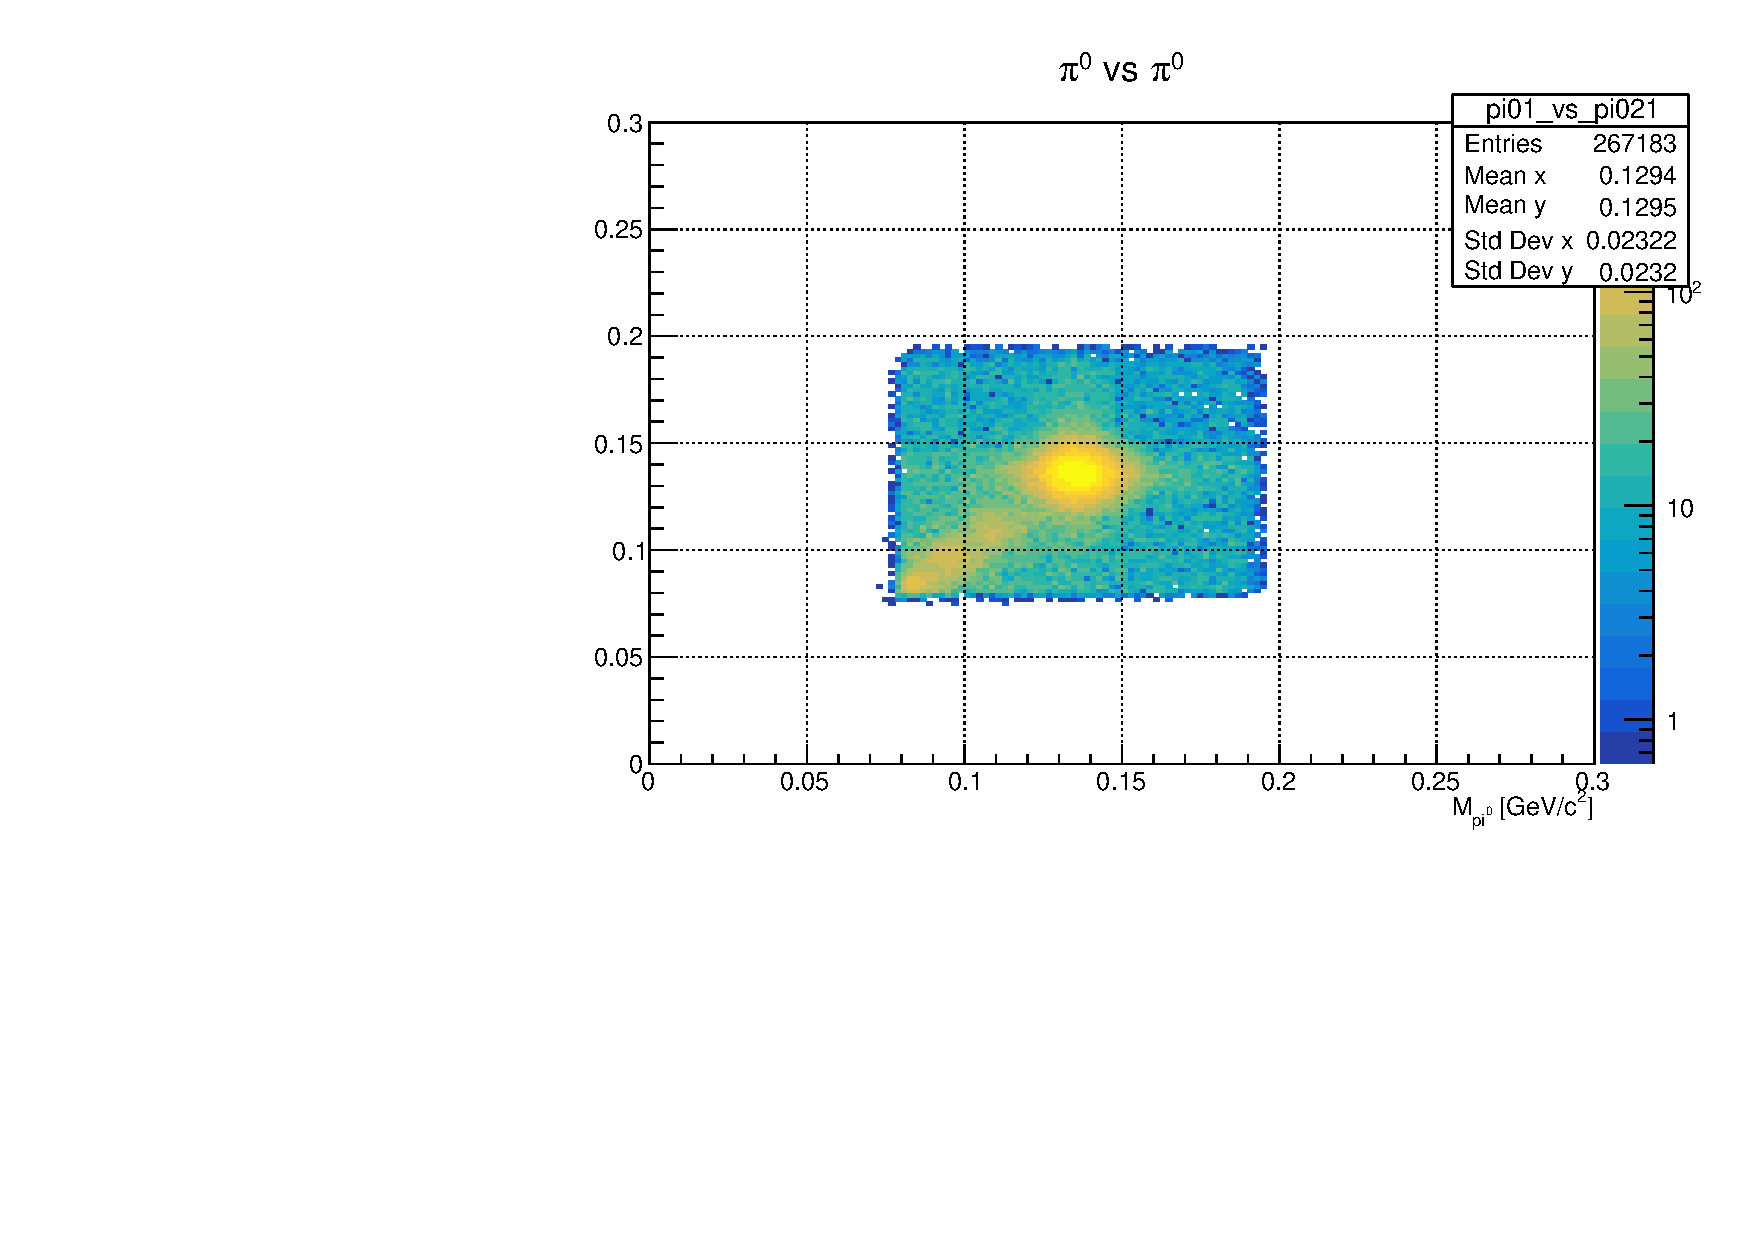
\includegraphics[width=4.75in]{figures/pi0VSpi0.pdf} \\
\centering
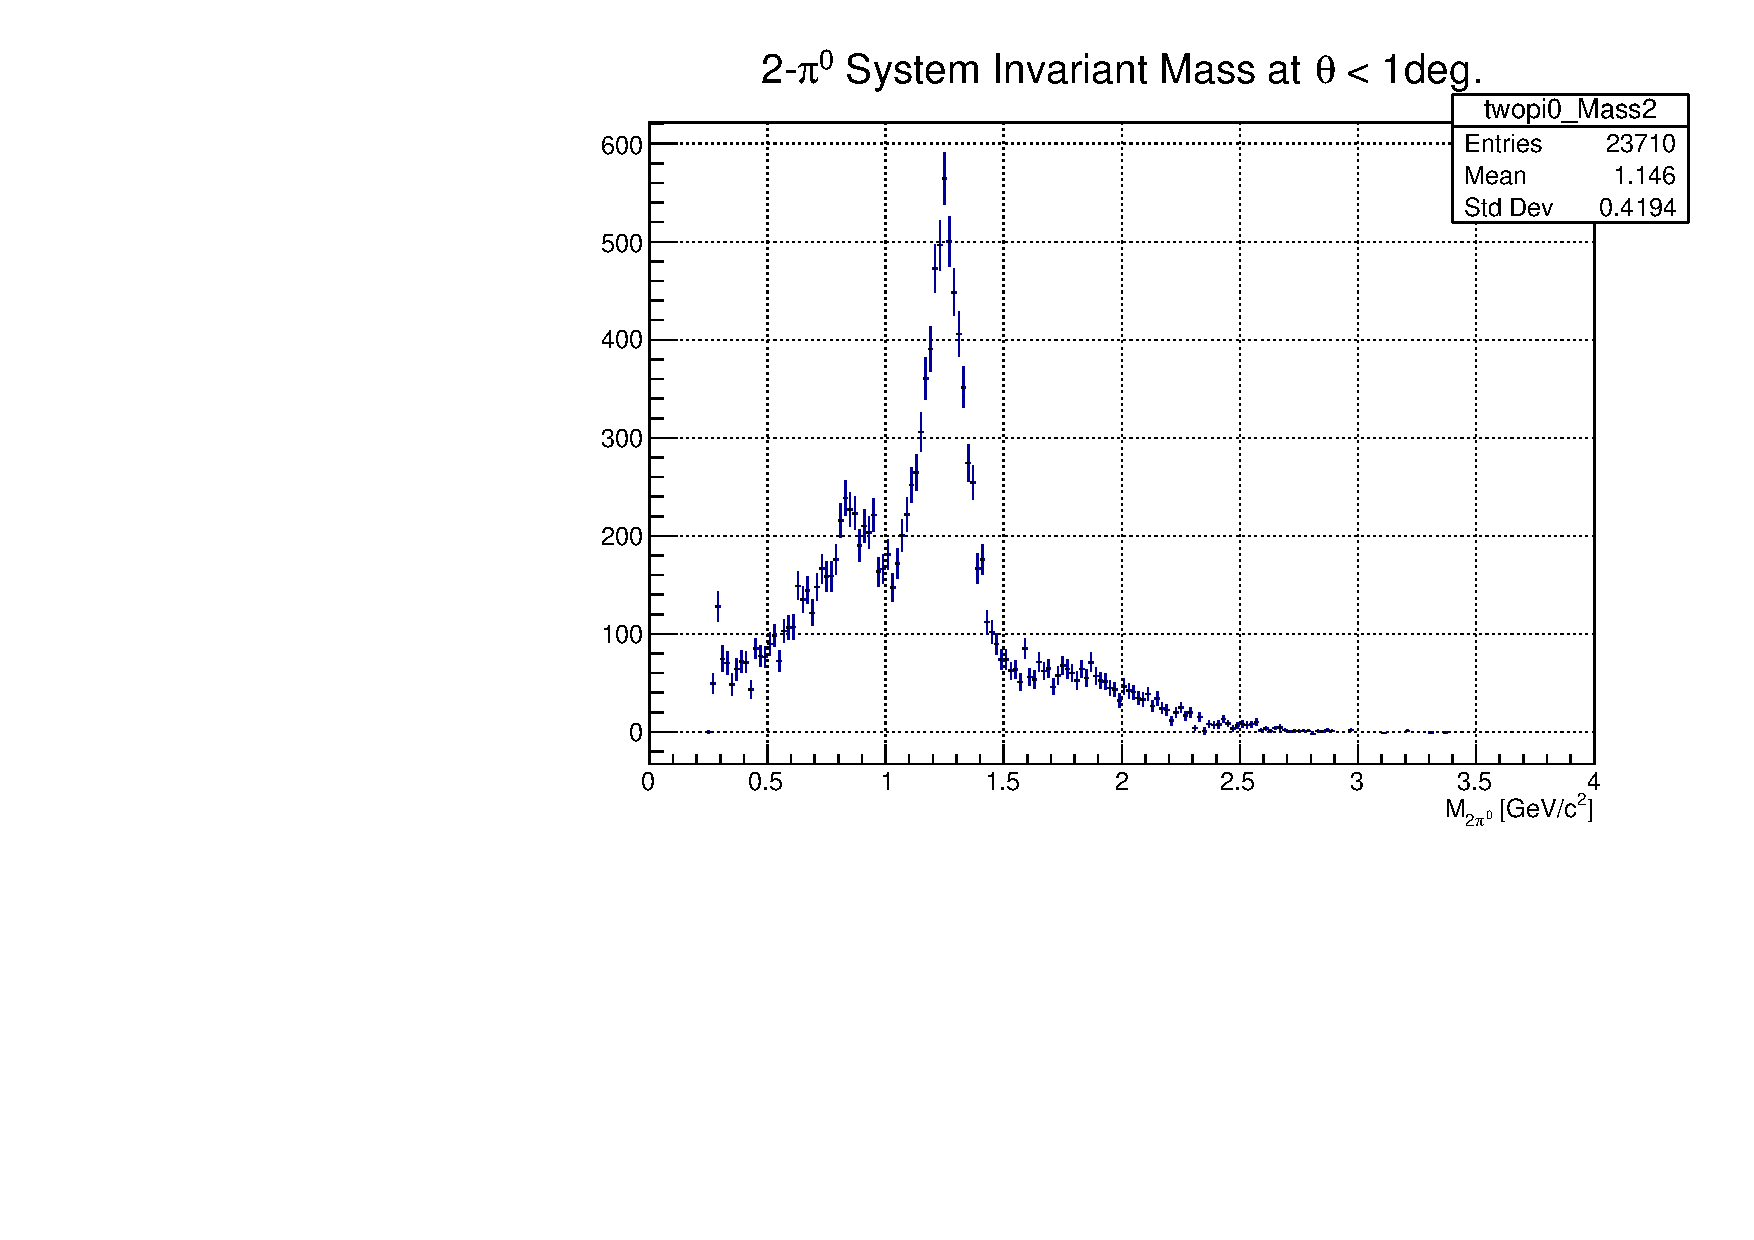
\includegraphics[width=4.75in]{figures/TwoPiInvMass.pdf}
\caption{Experimental distributions from the 2017 GlueX data set analyzed as $\gamma p\rightarrow \gamma \gamma \gamma \gamma\, (p)$ with a missing proton. Top: Two photon invariant mass of one pair vs the two photon invariant mass of the second pair. Bottom: 2$\pi$ mass distribution selecting events with the reconstructed photon pair masses close to the $\pi^0$ mass as  shown above. The plot also requires that the angle of the two pion system be less than 1 degree.
\label{fig:TwoPiInvMass}}
\end{figure}

The invariant mass distributions of two photon pairs each show a
strong $\pi^0$ peak, as shown in the top of
Fig.\,\ref{fig:TwoPiInvMass}. There are background events that fall
under the two $\pi^0$ peaks, which requires further study,
nevertheless, using the selection of photon pairs that reconstruct to
the $\pi^0$, we can plot the 2$\pi^0$ mass spectrum (bottom of
Fig.\,\ref{fig:TwoPiInvMass}). The mass spectrum has recognizable
features, in particular the prominent $f_2(1270)$ that decays to
$\pi^0\pi^0$ 85\% of the time. The structure at $M_{\pi\pi}\sim$0.8
GeV appears too low for the $f_0(980)$ and is present in a location
where the Crystal Ball data \cite{Marsiske:1990hx} shows a low
yield. The yield for $M_{\pi\pi}<$0.5 GeV is consistent within a
factor of two of the relative yield compared to the $f_2(1270$ peak in
the Crystal Ball data. This analysis demonstrates that these neutral
events can be analyzed in our detector under significant more
challenging circumstances than we anticipate for the Primakoff
experiment. In particular, for the Primakoff experiment, we will have
a point nuclear target that will allow valid geometrical constraints
and limit the amount of missing momentum in the reaction. This will
make the kinematic fitting more effective.

It is evident from top plot in fig.~\ref{fig:TwoPiInvMass} that a cut
on the invariant mass of one reconstructed $\pi^{0}$ will reduce the
background on the other $\pi^{0}$ significantly. This is shown in
fig.~\ref{fig:pi0yield} where a cut on the invariant of one $\pi^{0}$
significantly reduces the background in the other while keeping the
main signal mostly undisturbed.
\begin{figure}[htp]
\centering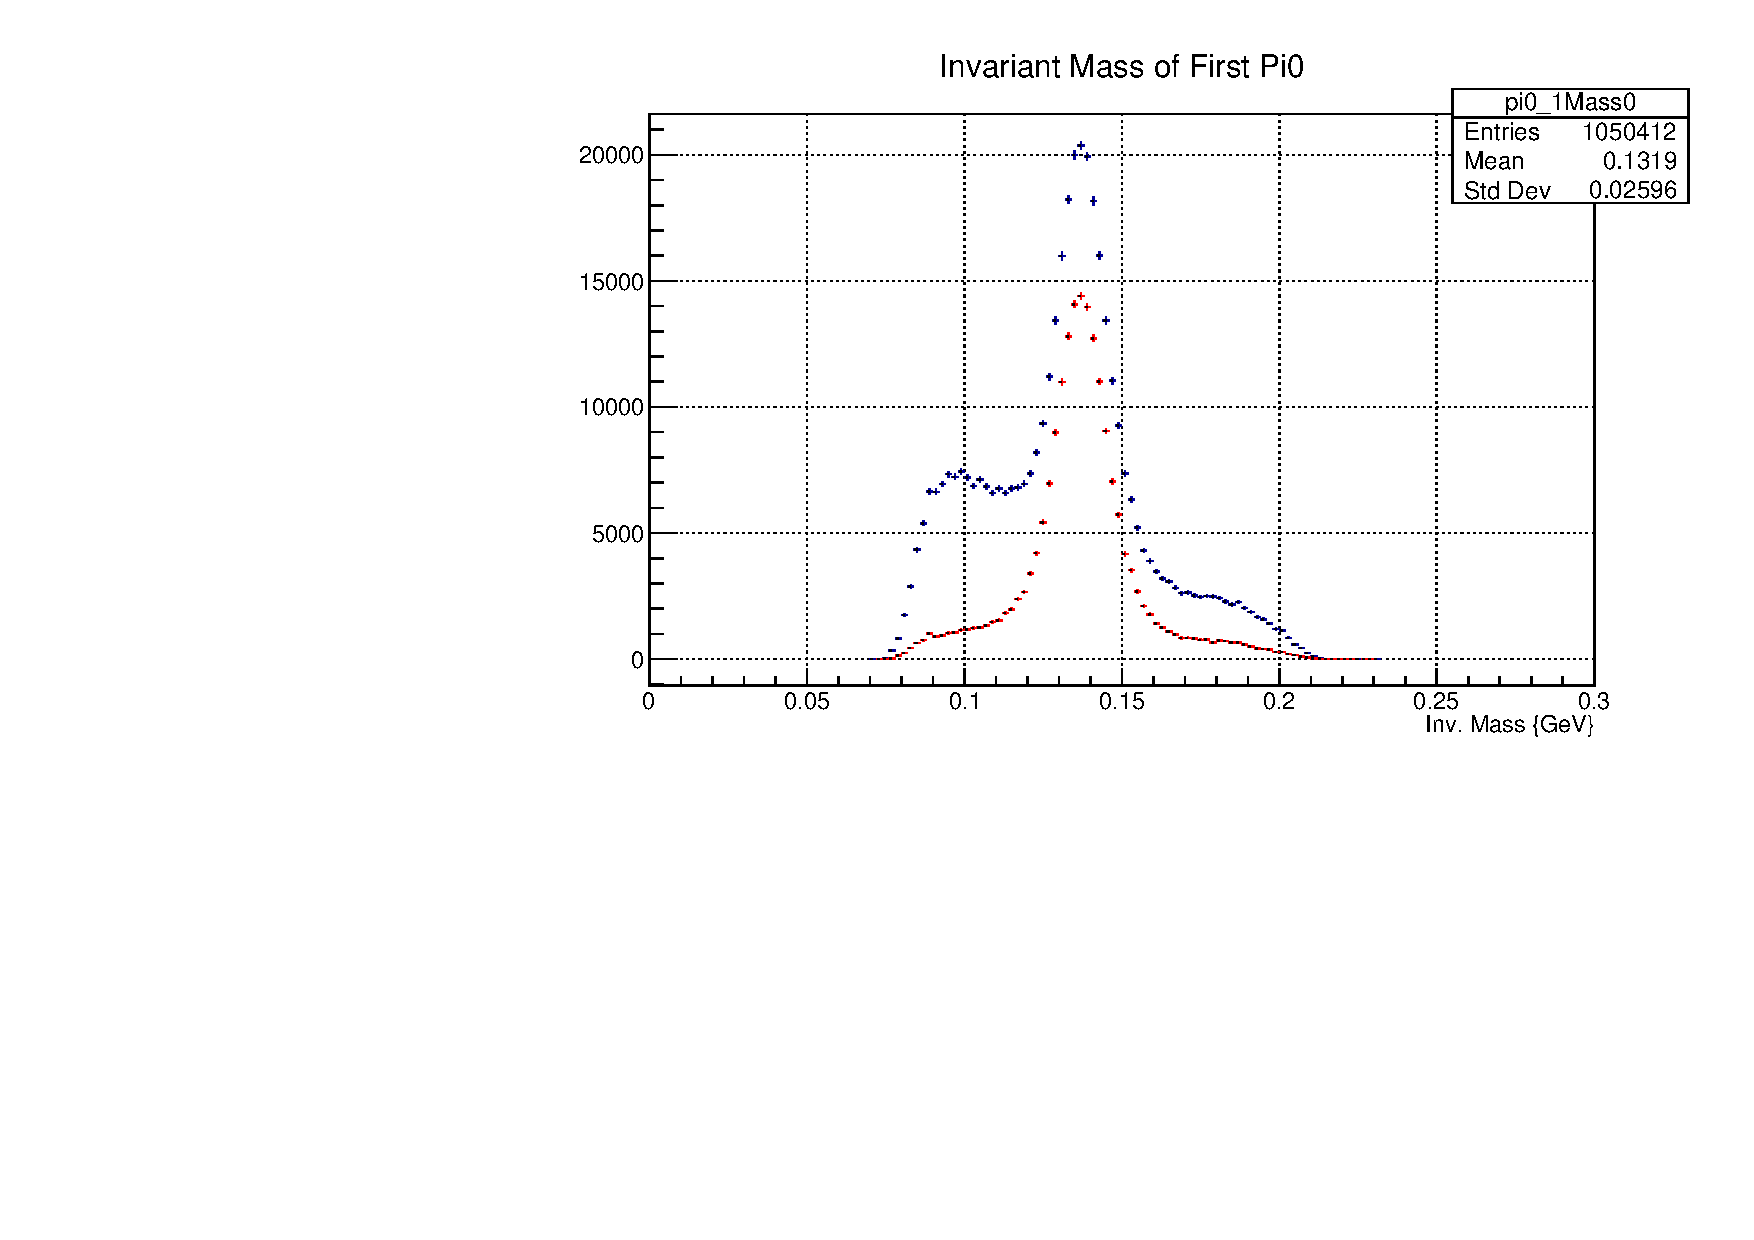
\includegraphics[width=4.75in]{figures/pi0_inv_mass_withpi02cut.pdf}
\caption{Invariant mass of the two photon system with(red) and without(blue) a cut on the invariant mass of the second pair of photons.
\label{fig:pi0yield}}
\end{figure}

These photons are detected by the lead-glass calorimeter and are the
main contribution to the resolution of the reconstructed $pi^{0}$
mass. A lead-tungstate calorimeter with a substantially better energy
resolution would yield a significant improvement in the signal to
noise ration as the width of the reconstructed $\pi^{0}$ would be
smaller by about a factor of 2.
